\chapter{Ứng dụng hỗ trợ biên tập}\label{app:application}
\FloatBarrier
\section{Kiến trúc dịch vụ và yêu cầu nhất quán khi suy luận}
Ứng dụng đưa gói PhoBERT vào quy trình nhập bài, đề xuất nhãn, rà soát và lưu phản hồi. Sáu dịch vụ trong Docker Compose gồm React/Vite UI, FastAPI API, dịch vụ mô hình gRPC, PostgreSQL, Redis và Dramatiq worker. UI dùng HTTP 5173, API 8000, dịch vụ mô hình gRPC 50051; lược đồ cơ sở dữ liệu \texttt{vnn} lưu bài, prediction, phản hồi, phiên và registry. Redis hỗ trợ hàng đợi, worker xử lý import hoặc recompute monitoring.
\AppDiagram
Dịch vụ mô hình nạp gói mô hình theo \texttt{app/artifacts/active.json}: trọng số PhoBERT, bộ mã hóa token được lưu cùng gói, hệ thống chuyên mục 20 lớp, Head--Tail 256, temperature và toàn bộ hệ số lớp. Khi khởi động, dịch vụ kiểm tra tệp, bảng ánh xạ nhãn và mã băm SHA của trọng số; mô hình được đặt ở chế độ đánh giá (eval), tắt dropout. Ba gói SVM/LR/BiLSTM là đối chứng offline, chưa là lựa chọn mô hình trong UI. Với container hiện tại, suy luận dùng CPU float32; notebook mạng nơ-ron dùng GPU BF16, nên logits sát ranh giới có thể khác nhỏ dù cùng quy tắc.

Ba vai trò Editor, Admin và Data Scientist có quyền tương ứng ở API. Phân quyền không chỉ dựa vào việc ẩn nút trong UI. Gói mô hình bao gồm thông tin mô tả và tokenizer cùng trọng số; chỉ có config/tokenizer trong clone mà thiếu trọng số không đủ để chạy dịch vụ. Các yêu cầu này giúp tránh mô hình nạp được tensor nhưng dùng sai nhãn hoặc sai tiền xử lý.

\FloatBarrier
\section{Quy trình dự đoán, đọc bài và sửa nhãn}
Editor nhập URL VietNamNet hoặc dán tiêu đề/nội dung. Dịch vụ kiểm tra đầu vào có văn bản sử dụng được, lưu nội dung đầy đủ và gọi inference; công việc bất đồng bộ có job ID để theo dõi. Lỗi tải và đầu vào rỗng không được thay bằng dự đoán giả. Các bài nhập trong app không tự được đưa vào tập dữ liệu notebook.
\begin{figure}[htbp]\centering
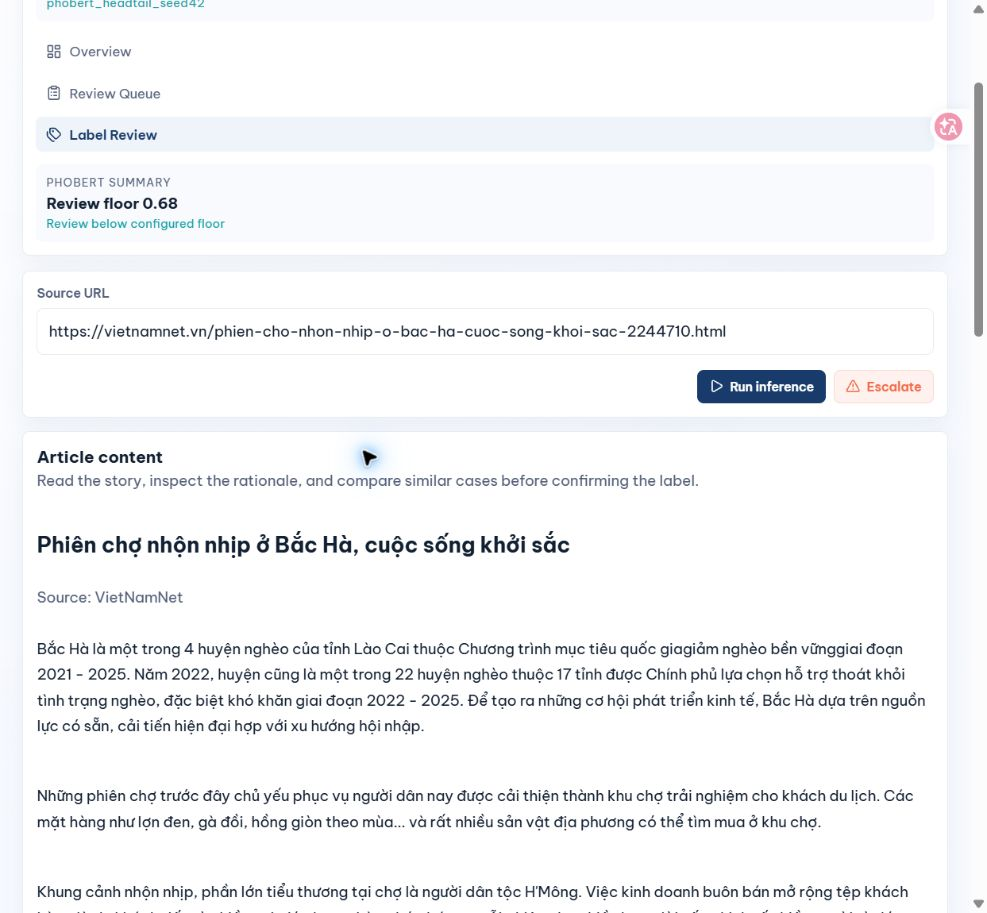
\includegraphics[width=.84\linewidth,height=.66\textheight,keepaspectratio]{assets/application/article_review.png}
\caption{Nội dung bài và URL nguồn trong màn hình rà soát.}\label{fig:app-review}\end{figure}
\begin{figure}[htbp]\centering
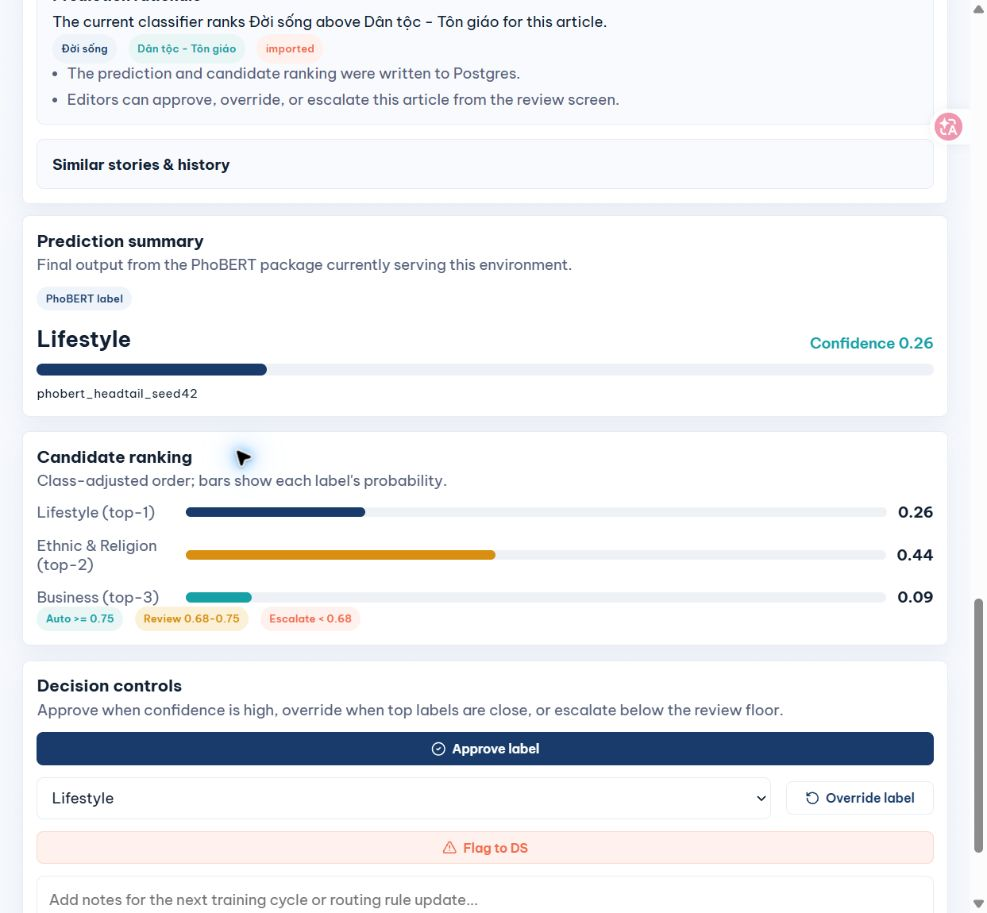
\includegraphics[width=.84\linewidth,height=.66\textheight,keepaspectratio]{assets/application/prediction_controls.png}
\caption{Nhãn gợi ý, độ tin cậy, các ứng viên và thao tác biên tập.}\end{figure}
Ví dụ ``Phiên chợ nhộn nhịp ở Bắc Hà, cuộc sống khởi sắc'' có nội dung du lịch, sinh kế và giảm nghèo. Mô hình chọn Đời sống với độ tin cậy khoảng 0.26, trong khi xác suất Dân tộc -- Tôn giáo khoảng 0.44. Điều này phù hợp với hệ số quyết định: nhãn xếp đầu theo $r=p/\tau$ có thể không có xác suất lớn nhất. Độ tin cậy thấp chuyển bài cho người xử lý chuyên sâu (escalate); không coi ví dụ này như một đánh giá test mới.
\ReviewDiagram
Ba thao tác biên tập là Approve (chấp nhận nhãn đề xuất), Override (chọn nhãn khác trong danh sách chuyên mục) và Escalate (chuyển bài khó để xử lý chuyên sâu). API từ chối approve với nhãn không phải top-1 hoặc khi chưa có prediction hợp lệ. Phản hồi gắn đúng prediction ID; suy luận lại tạo prediction mới, không tự chuyển phản hồi cho lần cũ thành nhãn tham chiếu của lần mới. Các khối từ khóa trên giao diện không phải lời giải thích đóng góp của attention.

\FloatBarrier
\section{Phân luồng và vận hành}
Chính sách cơ sở dữ liệu dùng độ tin cậy $p_{\hat y}(T)$: từ 0.75 là duyệt tự động; từ 0.68 đến dưới 0.75 là rà soát (review); thấp hơn 0.68 là xử lý chuyên sâu (escalate). Các ngưỡng phân luồng khác hệ số $\tau_c$ và khác margin trên $q=r/\sum r$. Thay ngưỡng không fine-tune mô hình, không ước lượng lại temperature và không tạo xác suất calibrated cho $q$.
\ReportFigure[.83]{assets/application/admin_ops.png}{Admin xem preview và điều chỉnh hai ngưỡng phân luồng của dữ liệu vận hành.}
Preview tính lượng bài trong từng luồng trước khi áp dụng chính sách. Offline selective prediction ở hình~\ref{fig:coverage} cho thấy đổi ngưỡng giảm khối lượng tự động nhưng không loại bỏ mọi lỗi. Accuracy trên nhóm giữ lại khác Accuracy toàn tập; threshold không phải bảo đảm an toàn hoặc SLA.
\ReportFigure[.86]{assets/evaluation/coverage_accuracy.png}{Tỷ lệ bài được giữ và Accuracy có điều kiện của nhóm đạt ngưỡng trên test; đây là mô phỏng offline.\label{fig:coverage}}
Danh mục phiên bản mô hình (registry) hiển thị thông tin mô tả, chỉ số offline, file tệp kết quả và trạng thái active. Upload kiểm tra path/tên, thông tin mô tả và khả năng nạp suy luận trước đăng ký. Kích hoạt kiểm tra gói mô hình, lấy khóa triển khai, thay manifest bằng thao tác \texttt{os.replace}, health check đúng run ID rồi cập nhật cơ sở dữ liệu. Nếu thất bại, mã nguồn phục hồi manifest cũ; cơ chế này chưa chứng minh an toàn giao dịch toàn hệ thống dưới mọi lỗi tiến trình.
\ReportFigure[.83]{assets/application/model_versions.png}{Danh mục phiên bản PhoBERT: phiên bản, hiệu chỉnh xác suất và kết quả offline từ tệp kết quả.}

\FloatBarrier
\section{Monitoring và Dataset Lab}
Chức năng giám sát ghép phản hồi với đúng prediction. Macro-F1 ở đây tính trên các nhãn quan sát được trong nhóm có phản hồi, không mặc định đủ 20 lớp. Các bài được chọn rà soát có thiên lệch, nên không đối chiếu trực tiếp số trên UI với Macro-F1 test offline. Điểm cảnh báo thay đổi dữ liệu kết hợp chênh lệch điểm giữa hai nhãn đầu và sai khác phản hồi theo quy tắc kinh nghiệm, chưa là kiểm định phân bố.
\begin{figure}[htbp]\centering
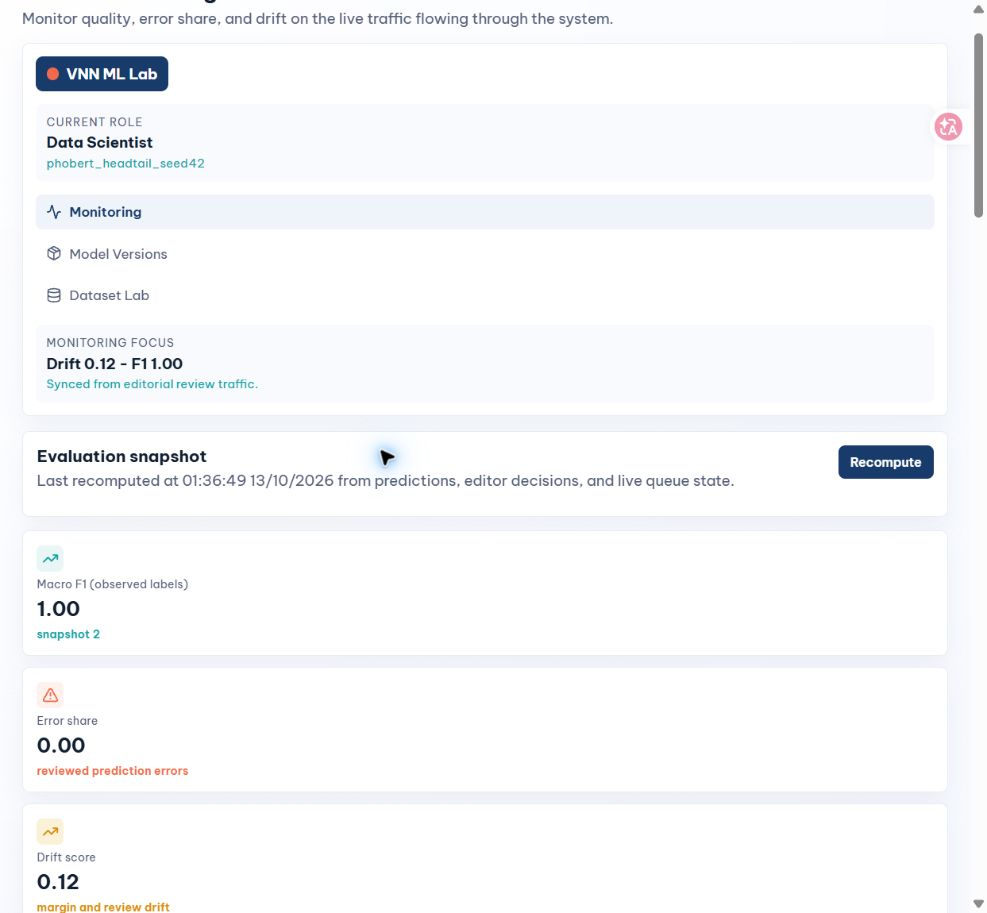
\includegraphics[width=.84\linewidth,height=.66\textheight,keepaspectratio]{assets/application/monitoring.png}
\caption{Monitoring theo phản hồi gắn với đúng prediction.}\label{fig:app-monitoring}\end{figure}
\begin{figure}[htbp]\centering
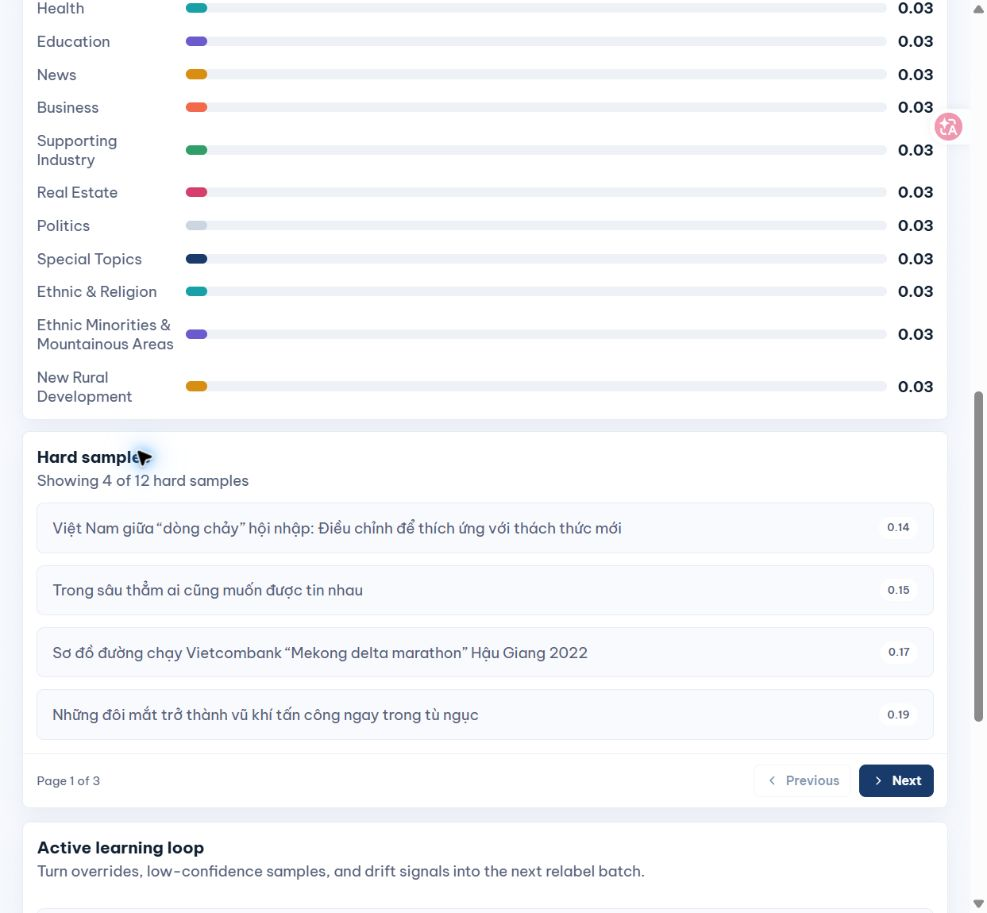
\includegraphics[width=.84\linewidth,height=.66\textheight,keepaspectratio]{assets/application/dataset_lab.png}
\caption{Dataset Lab: phân bố và ứng viên rà soát trong dữ liệu vận hành.}\end{figure}
Dataset Lab trình bày bài khó, độ tin cậy thấp và các bài cần xem xét lại nhãn. Hệ thống lưu phản hồi và job, chưa có vòng tự fine-tuning rồi tự triển khai bản lưu mô hình. Bản lưu cơ sở dữ liệu minh họa có 32 bài từ tập dữ liệu với dự đoán thật; phân bố được chọn để minh họa lớp và tình huống khó, không đại diện tập dữ liệu huấn luyện. Backup chứa schema ứng dụng, không chứa toàn bộ dataset và trọng số.

\FloatBarrier
\section{Kiểm chứng và giới hạn}
Các nguồn có thể kiểm tra lại gồm output notebook, gói active, source API/dịch vụ mô hình, ảnh giao diện và bản lưu cơ sở dữ liệu. Notebook giữ kết quả nạp lại tệp kết quả và suy luận kiểm tra trên validation; các điều kiện từ chối đầu vào rỗng, mapping sai, hiệu chỉnh xác suất không hữu hạn hoặc tệp kết quả thiếu nằm trong mã nguồn. Báo cáo không coi logic kiểm tra tồn tại như bằng chứng mọi testcase quá trình thực thi đã được chạy lại.

Kiểm tra trạng thái dịch vụ, phân quyền theo vai trò (RBAC), suy luận nhất quán, kích hoạt tệp kết quả, worker và văn bản rỗng là các nhóm kiểm chứng liên quan đến quy trình phân loại. Tài liệu kiểm chứng của bài tập lớn nêu 46 kiểm tra tự động, nhưng nhật ký từng trường hợp kiểm thử không được giữ trong bản dữ liệu hiện tại; vì vậy không dùng số đó làm chứng nhận test có thể tái kiểm toán. Ảnh giao diện chứng minh trạng thái minh họa đã lưu, không chứng minh accuracy hoặc khả năng hoạt động ổn định trong môi trường thực tế.

Triển khai của bài tập lớn giới hạn localhost. Môi trường có lưu lượng mới cần quản lý thông tin bí mật, mã hóa kết nối TLS, khả năng chịu tải và thời hạn lưu dữ liệu và đánh giá lỗi tự động theo từng lớp. Một bài nằm ngoài các chuyên mục được hỗ trợ vẫn có thể được gán nhãn với độ tin cậy cao; monitoring không cung cấp bộ phát hiện ngoài miền đã kiểm chứng. Các giới hạn vận hành này tách biệt với kết quả test của bốn mô hình.
